\documentclass{report}
\usepackage{graphicx}
\usepackage{tikz}
\usepackage{pgf-pie}
\usepackage{graphicx}
\usepackage{pgfplots} 
\pgfplotsset{width=7cm,compat=1.8} 

\begin{document}
\title{\LaTeX  Report on \textbf{``Toward a Mobile Phone Based Solution for Micro-credit in Rural Bangladesh"}}
\author{Rukshar Alam,1305031, and Md.Saqib Hasan,1305057\\
Bangladesh University of Engineering and Technology,BUET}
\date{\today}
\begin{figure}
\begin{center}
\includegraphics[scale=1]{buetlogo2.png}
\end{center}
\end{figure}
\maketitle
\newpage

\tableofcontents
\newpage

\chapter{Abstract}
The history of micro-credit in Bangladesh dates back to the 70’s just after the independence of our motherland. The purpose was to develop the socio-economic conditions of Bangladeshi rural communities, many of whom are always in dire need of credit to begin small scale economic activities.
But over the years microcredit has also accumulated a lot controversies\cite{1}. Many question its objectives, many consider it to be detached from reality. For research, surveys were conducted in Jamalganj , Sylhet. The results are quite interesting since they reflect  on the lack of success of Microcredit  project there. Mobile based technologies can go a long way to not only solve the problems pertaining to failure but also bring about a positive change in the rural communities under micro-credit project.
\newpage

\chapter{Introduction}
In the developing world many people do not have enough properties to pledge for a loan in the big banks. Such people can also be unemployed. Micro-credit or micro-loan can help them to alleviate poverty and also provide self-employment. As the name suggests, micro-loan is small loans who do not have credible credit history. Overall life quality can be improved by getting involved in micro-credit projects.\cite{2}
Micro-credit is included in the principles of modern economy after four decades of research. Grameen Bank, BRAC, etc. have made the micro-credit endeavour a success in Bangladesh and so they inspired other nations to take up such institutions. About 30 million people in Bangladesh  are beneficiaries of Micro-credit projects. Nearly 154 million loans have been provided to them by about 250 Micro-credit banks. \cite{3}
One of the important  concepts of Micro-credit is to improve the status of poor women. In order to do this women are given preference in these projects. So nearly 90 percent beneficiaries of the loans are women.\cite{4}
Dr. Muhammad Yunus is the founder of Grameen Bank and paved the way for micro-finance in Bangladesh. For these inspiring endeavours he won the Noble Peace Prize in 2006. 

 Many argue that micro-credit failed to lessen poverty in many developing regions in the world with reports of worsening conditions due to high interest rates, natural disasters etc. being regularly documented. \cite{5} \cite{6}
The paper has documented the results of surveys in Jamalganj area of Sunamganj district of Bangladesh.
Micro-credit organizations have constantly tried to improve the fate of the poor people there but failed most of the times. Data collection has been done through questionnaire. Data have been collected from those who partook in various micro-credit projects. After the analysis of the data gathered, the causes of frequent failure of micro-credit projects have been pointed out. To ensure success of the undertaken projects a  mobile technology based application has been proposed. This application is easy to use and understand.
\newpage

\chapter{Background Study}
Sapovadia documents the rigorous analysis of Micro-finance projects \cite{7}.  Though there are a number of limitations , the poverty stricken populace around the globe can indeed benefit from micro-credit scheme\cite{8}.  In the subcontinent , however, reports of failures have been extensively documented as well\cite{9}. There  are cases of severe mental duress as well as suicide of those who took the small loans but could not utilize to improve the lot \cite{10}. 
Mobile phone usage is on the rise around the world. In developing countries also there is a surge of cellular phone usage. A great many people from low-income households have at least one cell phone. So it is only natural that services that utilize mobile networks will gain popularity for there simplicity. In India a mobile technology based project called Avaaj Otalo by Stanford University, has greatly helped poor farmers. By using this service they can now ask about agricultural news and activities \cite{11}. 
Such projects can also be undertaken in Bangladesh too because mobile phones are quite popular in all the classes of people in this country both in the rural and the urban areas.
In order to gauge the success of large scale projects, small area based studies are constantly conducted. The same is done for Micro-finance projects. A popular example of such survey comes from Ghana, a country in the vast continent of Africa. The area was Lawra-Nandom District. There both men and women are involved in the same economic activities though there are cases of widespread gender discrimination when it comes to paying the employees. That paper not only addresses these issues but also provides solutions to put an end to gender gap by decreasing loan interest, ensuring availability of loan regardless of sex, etc.
UNESCO, AusAID and such international organizations can go a long way to use technology for spreading micro-credit in the world. Technology also helps a society for overall development. In \cite{12},  solutions are proposed to decrease the percent of poor people in the Pacific Island States by implementing technology.
\newpage

\chapter{Statistics}
The paper includes various data gathered about the people and Micro-Credit users at Jamalganj. All of these data are then presented in various statistical formats such as pie-charts,bar-graphs and tables.
All of these data conclude the following points:
\begin{itemize}
\item Most of the people in Jamalganj lack education.
\item Most of the people are involved in agriculture,especially on lands owned by others.
\item Many people are involved in the Micro-credit by their own will.
\item Maximum of them use a mobile phone
\end{itemize}
Here are the diagrams:

\begin{table}[h!]
  \centering
  \begin{tabular}{|l|l|l|}
  \hline
    \textbf{Age Group} & \textbf{Number of Microcredit Clients} & \textbf{Percentage}\\
    \hline
    1000-5000 & 17 & 56.67\\
    6000-10000 & 2 & 6.66\\
    11000-15000 & 3 & 10\\
    16000 Above & 8 & 26.67\\
    \hline
  \end{tabular}
  \caption{Loan Distribution of Micro-Credit Clients Respondents}
\end{table}

\begin{table}[h!]
  \centering
  \begin{tabular}{|l|l|l|}
  \hline
    \textbf{Age Group} & \textbf{Number of Microcredit Clients} & \textbf{Percentage}\\
    \hline
    20-30 & 8 & 26.67\\
    31-40 & 16 & 53.33\\
    41-50 & 4 & 13.33\\
    51 Above & 2 & 6.67\\
    \hline
  \end{tabular}
  \caption{Age of Micro-Credit Client Respondents}
\end{table}

\begin{table}[h!]
  \centering
  \begin{tabular}{|l|l|l|}
  \hline
    \textbf{Education Qualification} & \textbf{Number of Microcredit Clients} & \textbf{Percentage}\\
    \hline
    No-Formal Education & 6 & 20\\
    Primary & 8 & 26.67\\
    Middle & 10 & 33.33\\
    S.S.C & 6 & 20\\
    \hline
  \end{tabular}
  \caption{Education Qualification Distribution of Micro-Credit Client Respondents}
\end{table}

\begin{table}[h!]
  \centering
  \begin{tabular}{|l|l|l|}
  \hline
    \textbf{Family Member} & \textbf{Number of Microcredit Clients} & \textbf{Percentage}\\
    \hline
    1-2 & 1 & 3.33\\
    3-5 & 15 & 50\\
    6-8 & 13 & 43.34\\
    9-11 & 1 & 3.33\\
    \hline
  \end{tabular}
  \caption{Family Member Distribution of Micro-Credit Clients Respondents}
\end{table}

\begin{figure}[h!]
\centering
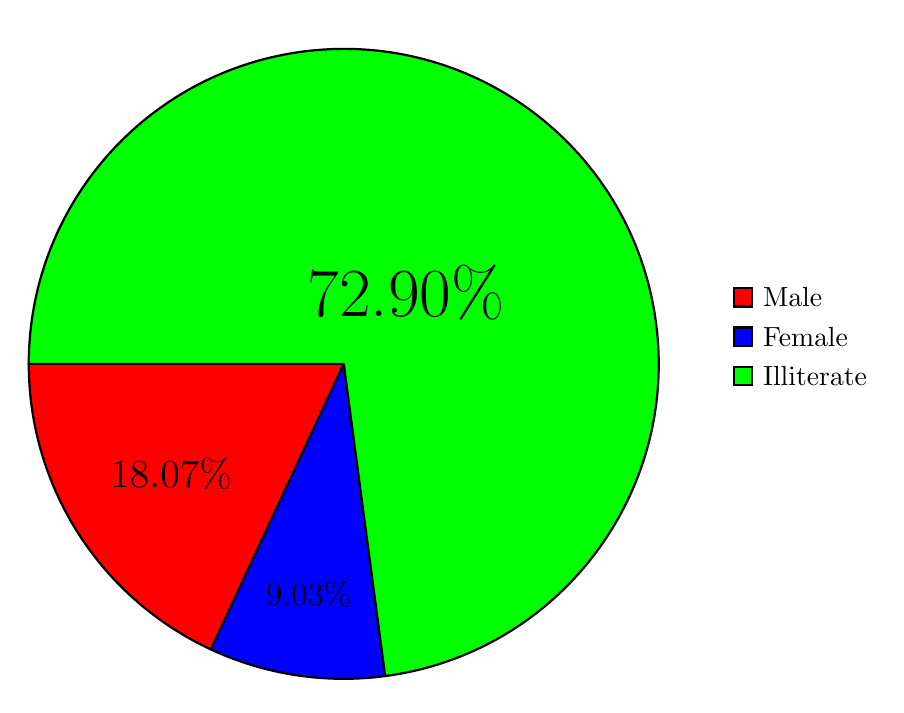
\begin{tikzpicture}[scale=1]

\pie[rotate = 180,radius=4,color = {red, blue, green},text=legend,scale font]{18.07/Male,9.03/Female, 72.90/Illiterate}

\end{tikzpicture}
\caption{Literacy rate of Jamalganj in Sylhet}
\end{figure}

\begin{figure}[h!]
\centering
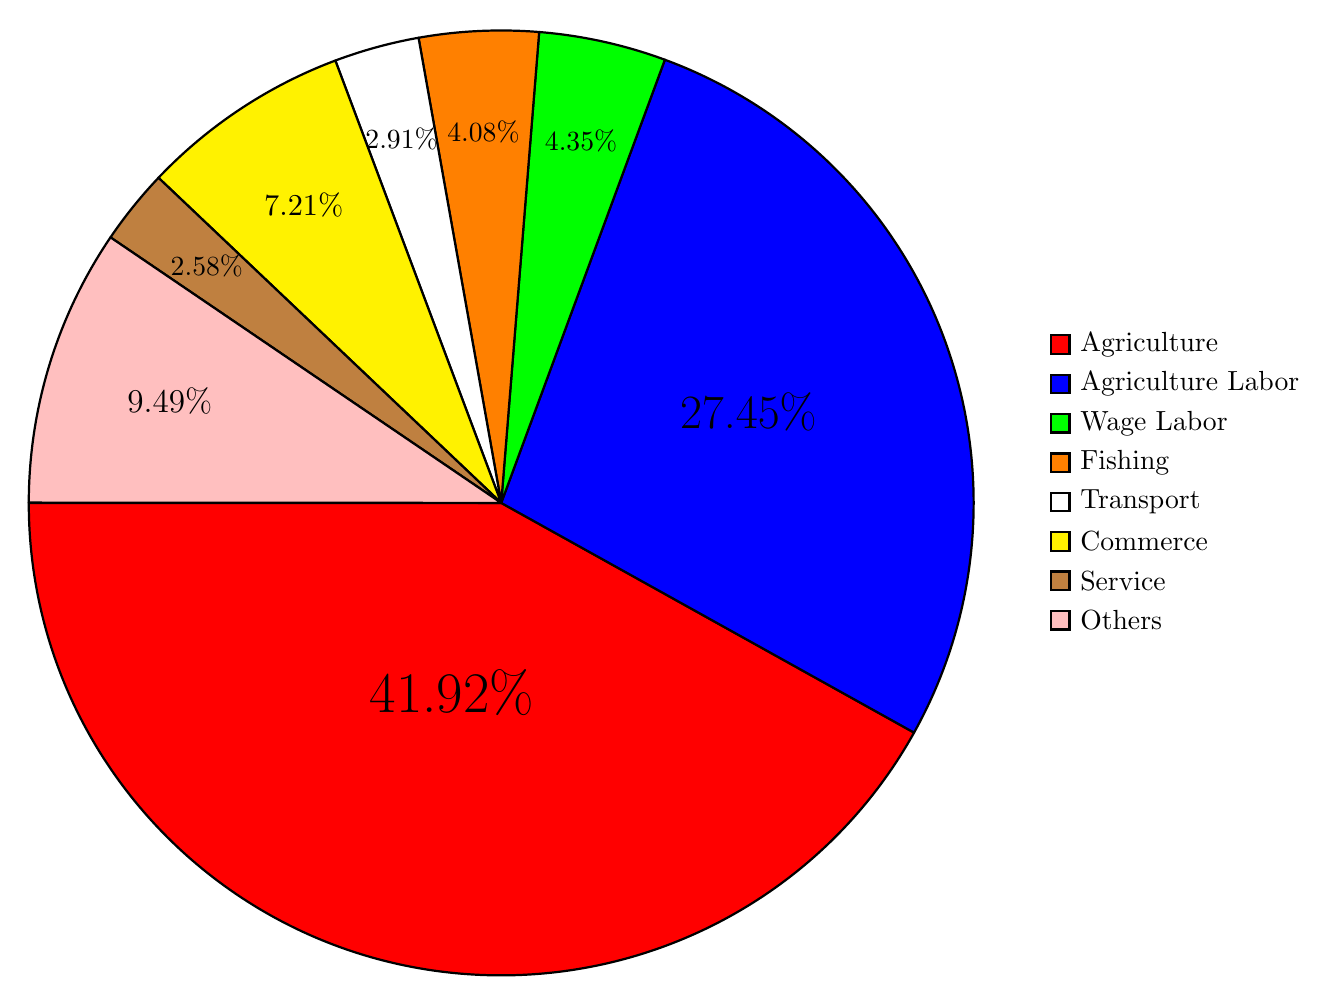
\begin{tikzpicture}[scale=1]

\pie[rotate = 180,radius=6,color = {red, blue, green,orange,white,yellow,brown,pink},text=legend,scale font]{41.92/Agriculture,27.45/Agriculture Labor,4.35/Wage Labor,4.08/Fishing,2.91/Transport,7.21/Commerce,2.58/Service,9.49/Others}

\end{tikzpicture}
\caption{Main occupations distribution of Jamalganj}
\end{figure}


\begin{figure}[h!]
\centering
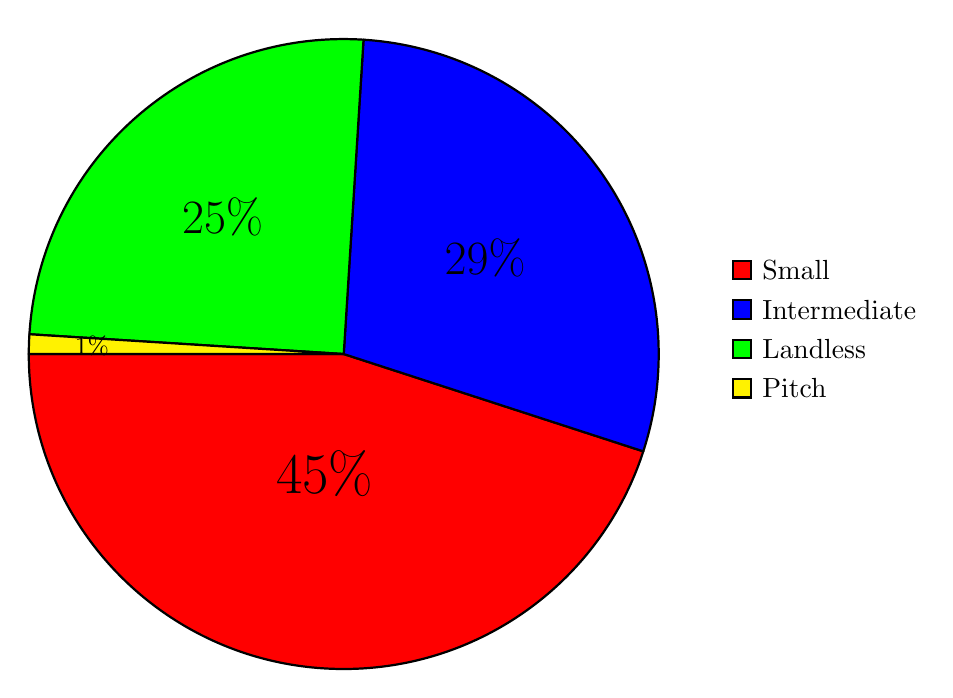
\begin{tikzpicture}[scale=1]

\pie[rotate = 180,radius=4,color = {red, blue, green,yellow},text=legend,scale font]{45/Small,29/Intermediate,25/Landless,1/Pitch}

\end{tikzpicture}
\caption{Land control in Jamalganj}
\end{figure}

\begin{figure}[h!]
\centering
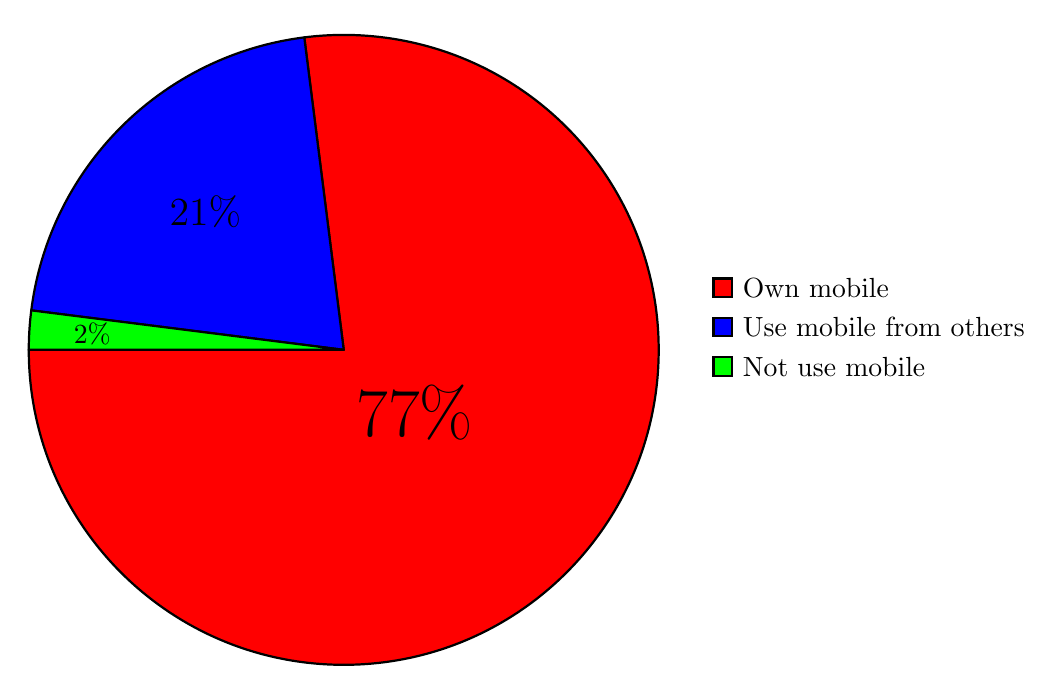
\begin{tikzpicture}[scale=1]

\pie[rotate = 180,radius=4,color = {red, blue, green},text=legend,scale font]{77/Own mobile,21/Use mobile from others,2/Not use mobile}

\end{tikzpicture}
\caption{Mobile user at Jamalganj in Sylhet}
\end{figure}


\begin{figure}[h!]
\centering
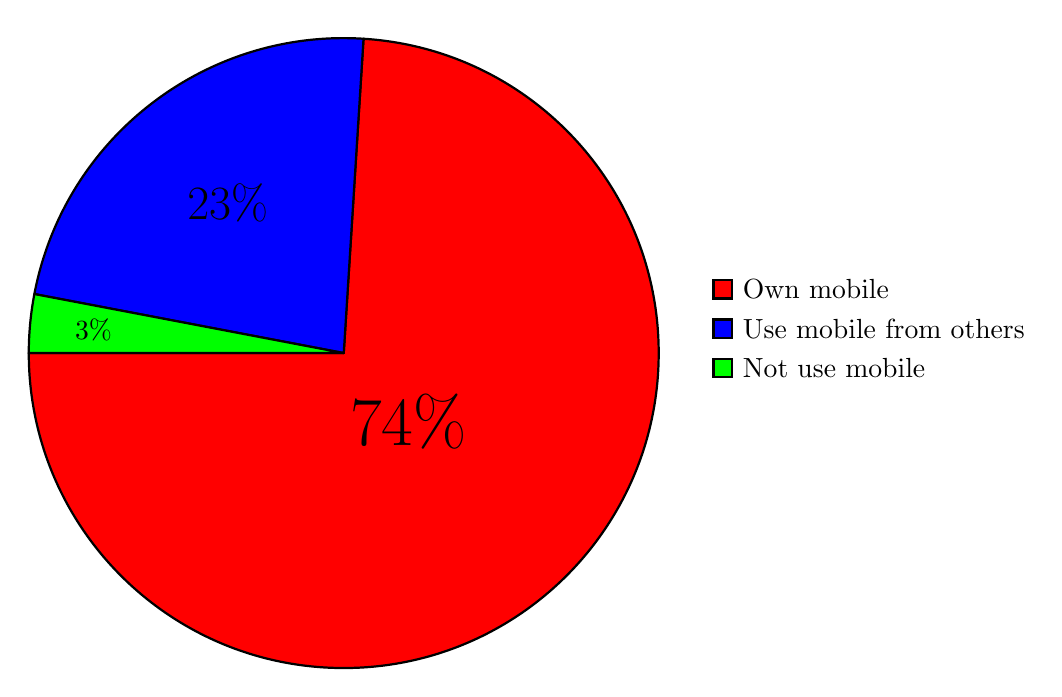
\begin{tikzpicture}[scale=1]

\pie[rotate = 180,radius=4,color = {red, blue, green},text=legend,scale font]{74/Own mobile,23/Use mobile from others,3/Not use mobile}

\end{tikzpicture}
\caption{Mobile user in micro credit clients}
\end{figure}

\begin{figure}[h!]
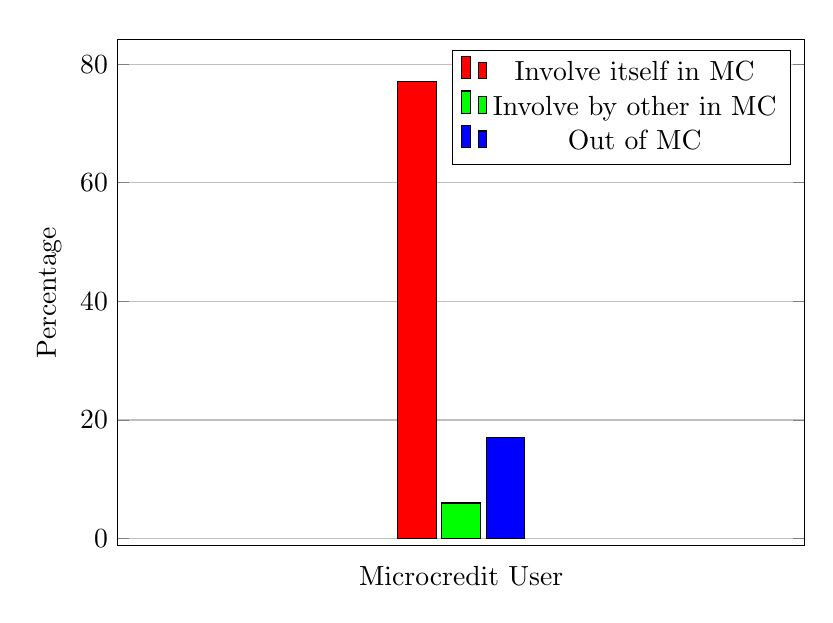
\begin{tikzpicture}
    \begin{axis}[
        width  = 0.85*\textwidth,
        height = 8cm,
        major x tick style = transparent,
        ybar,
        bar width=14pt,
        ymajorgrids = true,
        ylabel = {Percentage},
        symbolic x coords={Microcredit User},
        xtick = data,
        scaled y ticks = false,
    ]
            \addplot[fill=red]
            coordinates {(Microcredit User, 77) };
            \addplot[fill=green]
            coordinates { (Microcredit User,6)};
            \addplot[fill=blue]
            coordinates {(Microcredit User,17)};
         

        

        \legend{Involve itself in MC,Involve by other in MC,Out of MC}
    \end{axis}
\end{tikzpicture}
\caption{Micro-credit user at Jamalganj in Sylhet}
\end{figure}





\clearpage
\chapter{Some Problems Persisting in the Micro-Credit System}
The following points illustrate some of the problems still existing in our current system of micro-credit management:
\begin{enumerate}
\item Though there are many micro-credit organizations in   Bangladesh, there is  a general   lack of communication among them. They do not want to share user information. This environment of incoherence, rivalry and secrecy has allowed a group of people to take loans from multiple micro-credit banks without having to pay for the previous loans taken from other banks \cite{13}.
\item Micro-credit aims to eradicate poverty. Ironically the poorest of the poor are left out of its endeavours \cite{14}. The banks think  the poorest do not have capability to work out a plan to establish small businesses so  that they can pay the loans and the interests incurred \cite{15}.
\item According to the rules of micro-credit one has to pay the first instalment after the first week of loan sanction which is unrealistic for many borrowers. They are unable to generate any decent income in such a short span of time to pay the instalment. This creates an imbalance in the system \cite{16}.
\item Many borrowers do not have a solid plan on how to spend the loan. But they spend the money on personal matters which do not have any connections with the purpose of the loan.
\item Many accuse the interest rates charged on the loans provided is quite high. It can be as low as 11 percent but as high as 27 percent. Many poor people who have no other support and only dependent on such loans find it difficult to pay these interests in time and thus they become loan defaulters \cite{17}. 
\item Many men use their female relatives to gain access to loan because banks give out loans to women at a lower rate. If the men are unable come up with installments, the women have to bear the responsibilities.
\end{enumerate}
\newpage

\chapter{Solution Proposed by the Paper}
Since a lot of rural men and women use mobile phones,  a cellular phone based service can help greatly the problems mentioned in the paper. The solution suggested by this paper is text-message based so that even cheap mobile phones can be used.  Native bangla fonts and voice services can further simplify the process for the poor to gain easy access.
The solution involves two groups of people: the borrower and the seller of business utilities. They will be provided mobile accounts. A hopeful borrower must be physically present in the micro-credit organization premises to open an account. He/she is to bring a mobile phone along with proper identification papers. Giving loans and transactions are now controlled by the mobile account. Borrowers will have not case at hand. If they wish to purchase a required product from a registered seller, the transfer of money is done through their accounts.
\newpage

\chapter{Why the Proposed Solution?}
The solution proposed in the paper have been well thought and relies heavily on the use of technology. Still ,it was pointed as feasible and worth it due to the following reasons:
\begin{description}
\item[Proper use of money:] Since all the transactions are recorded in a database, any unprofitable expenditure will trigger warnings by notifying them.  Ensuring such well adjusted system of proper expenditure the clients are now unable to conduct unnecessary transactions. So now both the borrowers and the lenders will profit from the system which was quite hard in the past when only lenders seemed to profit but not the borrowers.

\item[Help to the poorest]The poorest cannot find employment in the villages and in the cities they may be involved in begging and criminal activities. Since the proposed solution ensures proper utilization of loans, the poorest can now also be eligible for borrowing money. Their involvement will reduce the social problems as well the economic ones.
BRAC have a scheme to sell mobile phones to the poorest in 12 month installments so that they can find it easier to finally purchase the means to make this project a success\cite{18}.

\item[Loan forwarded to clients:]There are many reported cases where a person uses another to get loans. This is a very risky behavior as any failure will result in pressure on the person actually took the loan. But in the proposed solution, the borrower must be present in the bank premises to verify mobile account.
Again the money being used by an unintended person is avoided as loan money can only be accessed through user mobile account.

\item[Risk of cash reduced:]Liquid money has many associated risks but now the whole transaction process has gone digital. Also password protection to mobile accounts and purchase through registered stores will decrease any chance of misuse.

\item[Fewer field workers:]Mobiles accounts of the borrowers can also be used to pay installments. This helps the banks to reduce their huge work force. Previously field workers were needed to get monthly installments from the borrowers.
\end{description}
\newpage

\chapter{The Algorithm/Process}
The algorithm is as follows:
\begin{itemize}
\item The hopeful borrower must be physically present in the bank to create an account. 
\item The filled up application and other documents are verified by the bank authorities.
\item Account information is inserted into database.
\item Directions are given to properly use the service.
\item Confirmation of account information is done through user mobile phone.
\item At the registered shops borrowers can purchase items by giving codes as input
\item Transactions along with their confirmation are done through the account while the sellers can withdraw the case
\item Prior to payments proper notifications are sent.
\item At load point the sales person documents borrowers account information for installments.
\item If needed short term training and maximum 16\% loan can be given to the borrower.
\end{itemize}
\newpage

\chapter{The Drawbacks of our Solution}
Even with such efficient and monitored micro-credit managment system, there comes various forms of drawbacks. Here are the major ones discovered by the research team:
\begin{description}
\item[Lack of education:] As most poor people are illiterate, getting them acquainted with the new solution will be difficult. This can solved by provided short term lessons on use of technology.
\item[Availability of shops:] it will be difficult to convince the shopkeepers to participate in the program since many of them lack the knowledge of technology. So they may be less interested in a system where they cannot get their hands on the money immediately. If their ignorance can be dispelled through awareness and inspiration, they will be more interested in participating in the project.
\item[New concept] Since cellular based service is a quite new phenomenon in Bangladesh , many current rules need to be altered to accommodate the proposed solution.

\end{description}
\newpage

\chapter{Conclusion}
Overall by taking a sample area to study the failure of microcredit system and coming up with a solution involving  widely used cellular technology, we can say the paper is ingenious.
\newpage

\begin{thebibliography}{13}
\bibitem{1}
Richard Rosenberg, Does Microcredit Really Help Poor People?, January
2010.
\bibitem{2}
Microcredit, http://en.wikipedia.org/wiki/Microcredit, as on June 2011.
\bibitem{3}
Statistics of MFI in Bangladesh, http://www.bangladesh-bank.org/ fnansys/
mfi.php as on June, 2011.
\bibitem{4}
Hossain, M. Credit for the Alleviation of Rural Poverty: The Grameen
Bank in Bangladesh, Report No. 55. IFPRI. Washington DC, 1988
\bibitem{5}
Banerjee, Abhijit, Esther Duflo, Rachel Glennerster, and Cynthia Kinnan.
2009. The miracle of microfinance? Evidence from a randomized
evaluation. Cambridge, Mass.: MIT Poverty Action Lab, May.
\bibitem{6}
Rutherford, Stuart. 2000. The Poor and Their Money. New Delhi: Oxford
University Press/India.
\bibitem{7}
Sapovadia, Vrajlal K., ”Micro Finance: The Pillars of a Tool to Socio-
Economic Development”, Development Gateway, SSRN, 2006.
\bibitem{8}
Jonathan Morduch\&Robert F. Wagner Graduate Analysis of the Effects
of Microfinance on Poverty Reduction, School of Public Service, New
York University, 4 Washington Square North, New York, NY 10003.
\bibitem{9}
Danger of Microcredit, http://news.guelphmercury.com/News/article
/724096, as on June, 2011.
\bibitem{10}
Suicide among microcredit clients, http://www.bloomberg.com/news/
2010-12-28/suicides-among-borrowers-in-india-show-how-men-made-amess-
of-microcredit.html, as on June, 2011
\bibitem{11}
Avaaj Otalo, http://www.stanford.edu/ neilp/pubs/
chi2010 patel.pdf
\bibitem{12}
Syeda Sharmin, The Grameen Micro-credit System and the Prospects of
Mobile Cellular Phones, in Fiji, Papua New Guinea, Samoa and Tonga.
\bibitem{13}
The University of Asia Pacific conference,16/06/2011, with ASA.
\bibitem{14}
Hashemi, S. M. and L. Morshed Grameen Bank: A Case Study. In Who
Needs Credit? Poverty and Finance in Bangladesh (eds) G.D. Wood and
I. Sharif, University Press Limited, Dhaka and Zed Books, UK. 1997.
\bibitem{15}
Microcredit for the Poorest, http://womenmicrocredit.wordpress.com, as
on June, 2011.
\bibitem{16}
The First Loan Payment of Microcredit, http://www.connexions.org/
CxLibrary/Docs/CX6992-MeadeMicrobank.htm, as on June, 2011.
\bibitem{17}
Interest Rates of Microcredit Organizations, http://www.grameeninfo.
org/index.php?option=com content\&task=view\& id=26\&Itemid =0,
as on June, 2011.
\bibitem{18}
Buying Mobile in Installments, http://www.bracbank.com/PayFlex-
Program.php, as on June, 2011.

\end{thebibliography}

\end{document}